\chapter{Background}
\label{ch:background}

In this section, we give background information about recent development of NLP research as well as metrics we use for our experiments.
Transfer learning with language models achieve state-of-the-art results on text classification.
Thus we use them for our work.

\section{Transfer Learning in Computer Vision and Natural-Language Processing}

Transfer learning is a research problem about re-using computation resulting from one problem to another problem. The survey of Pan et al.~\cite{pan2010survey} gives an overview over field as of 2010. With the `third wave' of artificial neural networks, the field of machine learning changed dramatically and thus transfer learning as well. With AlexNet~\cite{NIPS2012_4824} dramatically outperforming all other approaches in the 2012 ImageNet challenge, it started the revitalization process of neural models. Besides technological progress, one reason for the sudden success were large publicly available annotated research datasets such as ImageNet~\cite{imagenet_cvpr09}.
More data allowed to train deep networks with more layers networks (`deep learning'). In addition, these datasets gave a new perspective onto transfer learning in computer vision (CV). Nowadays, pre-trained ImageNet models are available in many open source libraries. And it is extremely common to fine-tune only a fraction of the weights as demonstrated by Oquab et al.~\cite{Oquab_2014_CVPR}. Mostly, only the last layers are trained because the early layers only learn very basic features such as edges as shown by Yosinski et al.~\cite{Yosinski:2014:TFD:2969033.2969197}. Consequently, transfer learning in CV allows to apply large neural models with millions of parameters even on small dataset sizes.

While in CV transfer learning is pre-dominate it was not used as often in NLP. There has been some progress however. Word2vec~\cite{Mikolov:2013:DRW:2999792.2999959} introduced word embeddings that are trained on large corpora in order to project words into a vector space. The resulting embeddings can be used on other task since they bring `meaning' to text. The idea of pre-trained word embeddings was especially popularized by pre-trained FastText embeddings available in 157 languages~\cite{grave2018learning}. FastText embeddings~\cite{TACL999} are adapting the idea of Word2vec but take sub-word information into consideration. However, the effect of word embeddings for neural networks is limited due to the following reasons: First, since one word can have multiple meanings (polysemy) a single vector is not enough to characterize it. For instance, `bank' can describe a financial institution or an embankment. The true meaning in a sentence can only be inferred by considering the context. Second, the message of a sentence can also depend on the context. Irony or satire are hard or impossible to grasp when only looking at individual words. Third, when using embeddings with neural networks, typically the embedding is used only for the first layer. Subsequent, deeper layers do not have access to the `meaning' of a word that was injected through the word embeddings.

A successor of word embeddings are text representations derived from language models. First we give background information on language models and where they were used originally.

\section{Language Modeling}

The research problem of creating a language model (LM) is, as the name suggests, about abstracting an entire natural language into a model.
Instead of formulating rules to describe the construction of a language, the model should capture it by showing a collection of natural language text. There are different ways of defining the problem. One can work on the level of sentences, word n-grams, words, sub-words or characters. We focus on words in this section. We also limit ourselves to modern neural network models since they greatly outperform traditional approaches.
For a comprehensive introduction, the interested reader is advised to read Chapter~9 of the book by Goldberg and Hirst~\cite{Goldberg:2017:NNM:3110856}.
Bengio et al.~\cite{Bengio03aneural} define LM in their seminal work as follows:
\begin{equation*}
 P(w_{1}^{T})=\prod_{t=1}^{T} P(w_t|w_{1}^{t-1})
\end{equation*}
where is the $t$-th word, and writing sub-sequence $w_{i}^{j} = (w_{i}, w_{i+1},\ldots, w_{j-1}, w_{j})$. This means that the probability of a word depends on all previous words. All previous words can mean a lot of words when the LMs, i.e., is trained on books. For the purpose of simplification, the first approaches worked with a fixed size window. In another groundbreaking work, Mikolov et al.~\cite{conf/interspeech/MikolovKBCK10} used a recurrent neural network (RNN) to circumvent the fixed window size and Sundermeyer et al.~\cite{Sundermeyer2012LSTMNN} successfully applied LSTMs~\cite{Hochreiter:1997:LSM:1246443.1246450} to language modeling. LSTMs are a powerful variant of RNN because they can capture long-term dependencies in sequences but as well `forget' previous input sequences. However, since LSTM are strong but contain a lot of parameters, they are known to overfit. Merity et al. introduced AWD-LSTM~\cite{merityRegOpt} that use a lot of regularization to overcome overfitting. As of this writing, AWD-LSTM variations still hold various state-of-the-art results on LM competition datasets\footnote{\url{http://nlpprogress.com/english/language_modeling.html}}.

LMs are used, e.g., for spell correction, optical character recognition, keyword prediction, or speech recognitions. As a byproduct they also embody a text representation that considers longer sequences of text. This is presented in the next section.

% mb remove
\newpage

\section{Transfer Learning with Language Models}
\label{sec:bgrd_tlwlm}

The idea of using LMs for text representation is not fundamentally new. As early as 2008, Collobert and Weston~\cite{Collobert:2008:UAN:1390156.1390177} demonstrate how they used LM as an auxiliary task for other downstream tasks. But only the ELMO (``Embeddings from Language Models'') embeddings by Peters et al.~\cite{peters2018deep} about ten years later popularized the idea. The basic principle works as follows.
The first task is to train a LM on a large text corpus.
The text does not require special annotations, although the arrangement of words in a text is a type of annotation itself. In such a manner, the model has to learn the nuances of a language over long sequences of text. After training a LM, its capabilities are transformed to other tasks such as text classification. The ELMO embeddings consider only parts of the internal state of the LM for further usage. Other approaches, i.e., ULMFIT~\cite{howard2018universal}, adopt the whole trained LM directly and only adds additional layers. ULMFIT will be explained more in detail in the next section. Both use LSTMs for the LM but ELMO operates on character level. There are two approaches based on the Transformer architecture~\cite{NIPS2017_7181}: the OpenAI transformer by Radford et al.~\cite{radford2018improving, radford2019language} and BERT by Devin et al.~\cite{devlin2018bert}. BERT improves the OpenAI transformer by allowing the model learn a language forth and backwards at the same time. This requires a different formulation of the language model problem but this is beyond the scope of this brief overview. Abkib et al.~\cite{akbik_contextual_nodate} use a character-aware LSTM-based LM to transfer-learn to named entity recognition. Peters et al.~\cite{peters_dissecting_2018} investigate the different capabilities of LMs. They show, i.e., that language models learn part-of-speech tagging implicitly. However, LM are not the only way to create context-aware text representation \cite{D18-2029, mccann2017learned}.
 But the current results suggest that they are superior.

\section{ULMFIT}

ULMFIT by Howard and Ruder~\cite{howard2018universal} is the acronym for ``Universal Language Model Fine-tuning for Text Classification''. As of this writing, the approach holds multiple state-of-the-art results on text classification\footnote{\url{http://nlpprogress.com/text_classification.html}} and sentiment detection\footnote{\url{http://nlpprogress.com/sentiment_analysis.html}}, i.e., on the IMDb dataset~\cite{maas2011learning}. Since publication, similar models such as the aforementioned BERT achieve state-of-art results on question answering. ULMFIT even with magnitude less parameters, is still undefeated for text classification.
In the ULMFIT paper, the authors point out that fine-tuning a LM to a smaller dataset is the crucial part.
LMs consist of millions of parameters and when training them on few samples, information may get lost fast (``catastrophic forgetting'').
 They use three techniques to circumvent it.
One technique they use is \textit{discriminative fine-tuning}.
It is about assigning different learning rates for each layer.
The earlier the layer in the neural network (closer to the input), the smaller the learning rate should be. In general, earlier layers learn fundamentals of the data while latter layers learn high-level features~\cite{Yosinski:2014:TFD:2969033.2969197}.
Another method used is \textit{cyclical learning rates} proposed by Leslie Smith~\cite{smith2017cyclical}.
Smith points out, that networks can be trained in less epochs by changing the learning rate of over time.
 Howard and Ruder argue that it is important to not fine-tune the LM for many epochs to avoid catastrophic forgetting and overfitting.
 Finally, they \textit{gradual unfreeze} the layers.
 Freezing layers means to not update the weights of certain layers.
 So unfreezing makes them trainable again.
 This special approach means that they do not unfreeze all layers at once.
 Instead, they progressively unfreeze layers starting from the final layer. So first, only the last layer is trained.
 Second, the last layer and second-last layers and so forth until the model is fully unfrozen.
 The authors state that only by the combination of these techniques, they could achieve high-scoring results.
 For the LM architecture, they use the already mentioned AWD-LSTM.
  First, they train a LM on a collection of high-quality English Wikipedia articles \textit{Wikitext103}\footnote{\url{https://blog.einstein.ai/the-wikitext-long-term-dependency-language-modeling-dataset}}~\cite{wikitext103}.
 After the general training of the LM, it requires fine-tuning to the specific domain.
 The LM is not powerful enough to hold the knowledge of the complete English language.
 Since language is different in each domain, they have to fine-tune the LM to the target domain.
 Then as the final step, a classifier is trained. For this, the LM architecture is augmented with two additional blocks of fully connected layers. The two different model architectures are visualized in Figure~\ref{fig:ulmfit_archi}.

\begin{figure}
    \centering
    \subfloat[]{{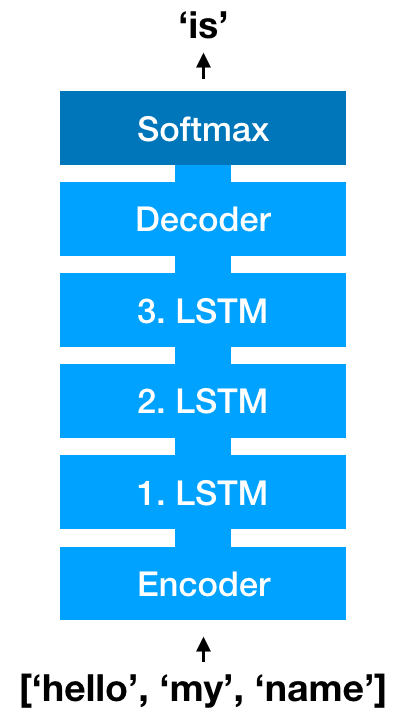
\includegraphics[height=150pt]{images/background/arch1.png} }}
    \subfloat[]{{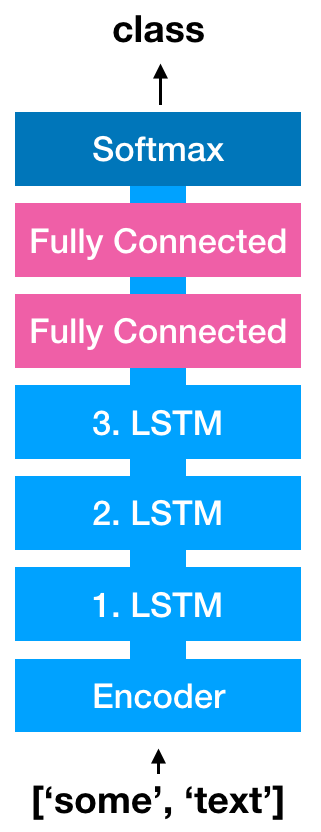
\includegraphics[height=173pt]{images/background/arch2_fixed2.png} }}
    \caption{The two different ULMFIT architectures. In Subfigure~(a) is the LM with a decoder to predict a news word. In Subfigure~(b) is the decoder replaced with two fully connected layers to predict a sample's class.}
    \label{fig:ulmfit_archi}
\end{figure}

The authors claim that even with only a small amount of annotated data, the classification achieves high results. Figure~\ref{fig:bgrd_ulmfit_res} demonstrates this at the example on IMDb movie reviews. This strength is particularly useful for newspaper, since resources to annotate data are scarce.

\begin{figure}
  \begin{center}
    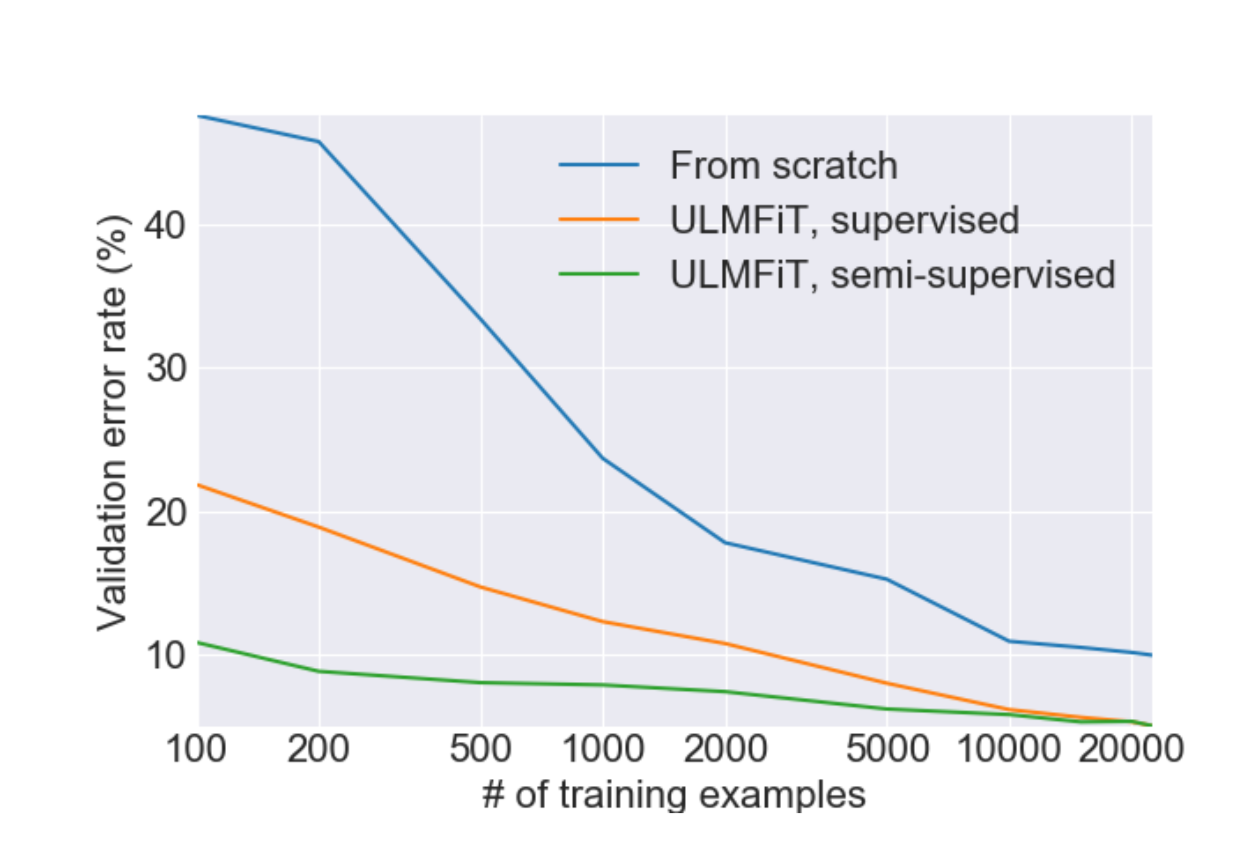
\includegraphics[width=0.6\textwidth]{images/background/ulmfit_results.png}
  \end{center}
  \caption{Validation error rates (lower is better) for ULMFIT on IMDb reviews. Semi-supervised means the LM is only fine-tuned on the according number of training samples whereas semi-supervised the LM is fine-tuned on all available samples. The figure was taken from the original paper~\cite{howard2018universal}.}
   \label{fig:bgrd_ulmfit_res}
\end{figure}

An implementation of ULMFIT is available in the Python deep learning library FastAI\footnote{\url{https://docs.fast.ai/text.html}} which itself is built upon PyTorch\footnote{\url{https://pytorch.org}}. It varies slightly from the original publication. The cyclical learning rate was originally not part of the paper but now the authors consider it as an integral part of the method.

%\newpage

\section{Classification Metrics}
\label{sec:metrics}

There is an abundance of metrics for classification. Sokolova and Lapalme give an overview~\cite{Sokolova:2009:SAP:1542545.1542682}. We briefly introduce those commonly used for news comment classification.

First, let us revisit precision, recall and $\text{F}_{1}$ score. With $tp$ as the number of true positives, $fp$ as the number of false positives, $tn$ as the number of true negatives, and $fn$ as the number of false negatives, precision and recall are defined as follows:

\begin{align*}
 \text{precision} &= \frac{tp}{tp+fp} & \text{recall} &= \frac{tp}{tp+fn} \\
\end{align*}

\newpage
The $\text{F}_{1}$ score is the harmonic mean of precision and recall:

\begin{equation*}
    \text{F}_{1} = 2 \cdot \frac{\text{precision} \cdot \text{recall}}{\text{precision} + \text{recall}}
\end{equation*}

In the original sense, precision and recall were compute in regard to one class. Hence, true positive and true negatives are calculated separately. But when using the metrics for classification, there is one drawback. The number of true negative samples are neither part of the precision nor recall formula.
Thus, these metrics do not lead to meaningful insights.
It is a problem when the majority class is treated as positive class.
In this case, it is easy to achieve high $\text{F}_{1}$~scores by simple always predicting the majority class (with a recall of 1 and high precision due being the majority class).
To overcome this, typically the scores are computed in regard to each class and then aggregated into a final score. There are three main types of aggregations: \textit{micro}, \textit{macro}, and \textit{weighted}\footnote{As implemented in the popular Python package scikit-learn.}. For \textit{micro}, the samples for true positives, false positives, etc., are counted across all classes and then the final score is computed.
For binary and multi-class classification, this is equivalent to the metric accuracy.
The accuracy is the share of samples there was assigned to the correct class.
For \textit{macro}, the scores are computed for each class separately and the intermediate scores are then averaged to a final score. \textit{Weighted} builds upon the macro-averaged score and weights them in respect to the number of samples per class.
Often micro and macro $\text{F}_{1}$~scores are used in conjunction to asses the quality of model.

Always using two metrics is cumbersome. To have a single metric that evaluates the performance of a model, we use Cohen's Kappa for this thesis.
Cohen's Kappa or short Kappa (or $\kappa$) was introduced by John Cohen~\cite{cohen_kappa_1960} and it was originally meant to measure the agreement among annotators.
However, it can be used as classification metric as well~\cite{ferri2009experimental,witten2005data}.

It is defined as follows:

\begin{equation*}
    \text{Kappa} = \frac{p_o - p_e}{1 - p_e}
\end{equation*}

$p_o$ is the observed agreement (accuracy) and $p_e$ is the expected agreement (accuracy by chance).
It takes into account whether classification results could happen randomly.
This is especially useful for imbalanced datasets, as it is often the case when working with real-life data such as news comments.
